\section{Results}

Table \ref{tab:res_prost} shows the obtained DSCs for the segmentation of the prostate when the three trained models are used for segmenting the GE and the Siemens dataset. The displayed DSCs are computed from the validation subset when the model is trained on the same dataset, and computed from the whole dataset when the model is trained from a different dataset. 

 \begin{table}[h]
    \caption{Prostate segmentation Dice Similarity Coefficients (DSC) obtained for the GE and Siemens MRI vendors datasets, from the
    tree trained models (GE, Siemens, and Combined). The DSC are obtained for the original MRI resolution, and for the high resolution images.}
    \begin{tabular}{lcc}
         \hline
          \textbf{Prostate Models} & \textbf{GE} & \textbf{Siemens }\\
         \hline
         %GE ROI/Original & $0.916\pm0.015$/$0.917\pm0.015$ & $0.465\pm0.198$/$0.466\pm0.198$ \\
         %GE & $\mathbf{0.917\pm0.015}$ & $0.466\pm0.198$ \\
         GE ROI/Original & $0.855\pm0.064$/$\mathbf{0.860\pm0.054}$ & $0.804\pm0.099$/$0.802\pm0.106$ \\
         \hline
         %Siemens ROI/Original & $0.261\pm0.119$/$0.276\pm0.130$ & $0.936\pm0.21$/$0.932\pm0.022$ \\
         %Siemens & $0.276\pm0.130$ & $\mathbf{0.932\pm0.022}$ \\
         Siemens ROI/Original & $0.262\pm0.118$/$0.288\pm0.139$ & $0.892\pm0.038$/$0.889\pm0.035$ \\
         \hline
         %Combined ROI/Original & $0.828\pm0.116$/$0.824\pm0.113$ & $0.909\pm0.032$/$0.907\pm0.031$\\
         %Combined & $0.824\pm0.113$ & $0.907\pm0.031$\\
         Combined ROI/Original & $0.830\pm0.112$/$0.827\pm0.109$ & $\mathbf{0.896\pm0.037}$/$0.892\pm0.036$\\
         \hline
    \end{tabular}
    \label{tab:res_prost}
\end{table} 
When the model is trained with examples from one dataset and used to segment prostates from scans of the same MRI vendor the average DSCs are: $0.855$ for GE and $0.892$ for Siemens. When the datasets are combined during training, the average DSC are: $0.830$ for GE and $0.896$ for Siemens.  The results obtained for the Siemens dataset are comparable with other methods for prostate segmentation. When the model is trained with examples from one MRI vendor and then used to process images from a different vendor, the resulting DSCs are low ($0.262$ and $0.804$).  This result exhibit how sensible the model is to subtle changes in the training dataset. It also displays the importance of testing how well deep learning architectures generalize to other MRI vendors.  

% Show some images
Figure \ref{fig:resseg} shows the middle axial slice for the lowest, median, and highest DSC obtained for prostate segmentation on the Siemens and GE dataset. In general, the DSC increases with respect of the volume size of the prostate, and images from the Siemens dataset have better resolution than GE, which may be reason of why the DSC are better in this dataset. 
\begin{figure}[h]
    \centering
    \includegraphics[totalheight=.4\textheight]{figures/Figure4.eps}
    \caption{Prostate segmentation for the cases with the lowest, middle, and highest 3D DSC for the Siemens (up) and GE (down) datasets. These segmentation are obtained with the \emph{Combined} network model.  }
    \label{fig:resseg}
\end{figure} 

Table \ref{tab:res_pz} shows the obtained DSCs for the segmentation of the PZ the three trained models.  The best DSCs of $0.797$ and $0.813$ for segmenting the PZ of the prostate are obtained when the model is trained using the combined dataset.  
 \begin{table}[h]
    \label{tab:res_pz}
    \caption{Dice Similarity Coefficients (DSC) between manual and CNN-generated PZ contours for GE and Siemens.The trained models are divided in: with (w) data augmentation (DA) and without (wo) DA.}
    \begin{tabular}{lcc}
         \hline
          \textbf{PZ Models} & \textbf{GE Dataset} & \textbf{Siemens Dataset}\\
         \hline
         GE ROI/Original & $0.767\pm0.093$/$0.759\pm0.089$ & $0.537\pm0.204$/$0.539\pm0.204$ \\
         %GE  & $\mathbf{0.74\pm0.09}$ & $0.40\pm0.22$ \\
         \hline
         Siemens ROI/Original & $0.591\pm0.223$/$0.591\pm0.219$ & $0.808\pm0.085$/$0.808\pm0.087$ \\
         %Siemens & $0.58\pm0.21$ & $\mathbf{0.78\pm0.08}$ \\
         \hline
         Combined ROI/Original & $\mathbf{0.797\pm0.093}$/$0.788\pm0.093$ & $\mathbf{0.813\pm0.079}$/$0.811\pm0.79$\\
         %Combined & $0.75\pm0.10$ & $0.78\pm0.09$\\
         \hline
    \end{tabular}
\end{table}

The average DSCs of all the PZ models are lower than the coefficients for segmenting the prostate, which implies that PZ segmentation is a more challenging task. The obtained DSC for segmenting the PZ with the \emph{Combined} model (0.788 and 0.811) are better than what we found in the literature for similar databases (0.60, 0.68, 0.62, 0.75) \cite{mooij_automatic_2018,toth_simultaneous_2013, chilali_gland_2016, hutchison_pattern_2012}. Figure \ref{fig:ressegpz} shows the middle axial slice for the lowest, median, and highest DSC obtained for the segmentation of the PZ on the Siemens and GE dataset. 
\begin{figure}[h]
    \centering
    \includegraphics[totalheight=.4\textheight]{figures/Figure5.eps}
    \caption{Peripheral zone segmentation for the cases with the lowest, middle, and highest 3D DSC for the Siemens (up) and GE (down) datasets. These segmentation are obtained with the \emph{Combined} network model.  }
    \label{fig:ressegpz}
\end{figure} 

% COMPARE WITH RESULTS FROM OTHER PLACES OF PZ AND SAY WE ARE THE BEST


% \begin{figure}[h]
%    \centering
%    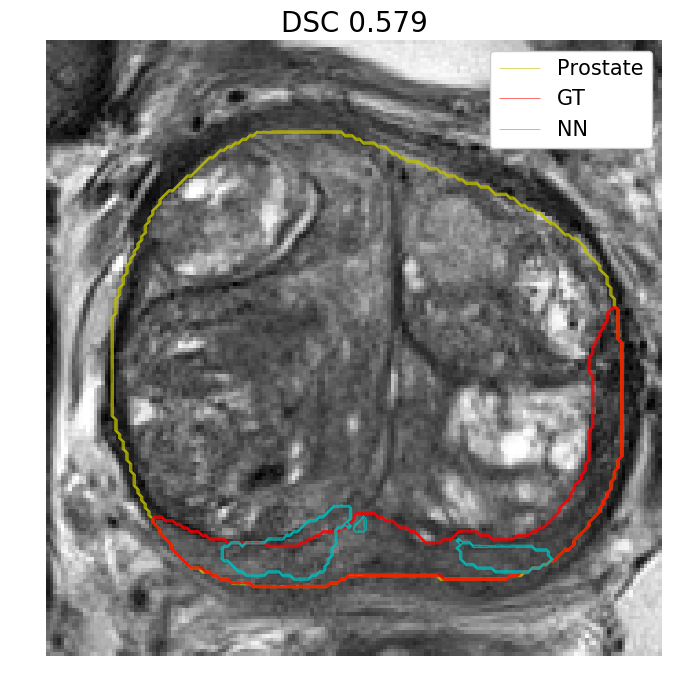
\includegraphics[totalheight=.2\textheight]{figures/results/PZ_Px_Challenge__P_yes_ROI_MIN_Case-0325.png}
%    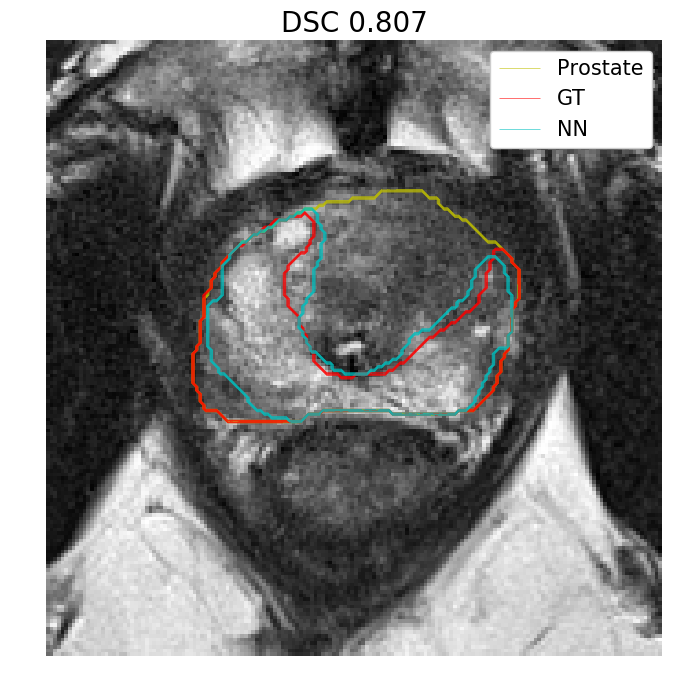
\includegraphics[totalheight=.2\textheight]{figures/results/PZ_Px_Challenge__P_yes_ROI_MEAN_Case-0319.png}
%    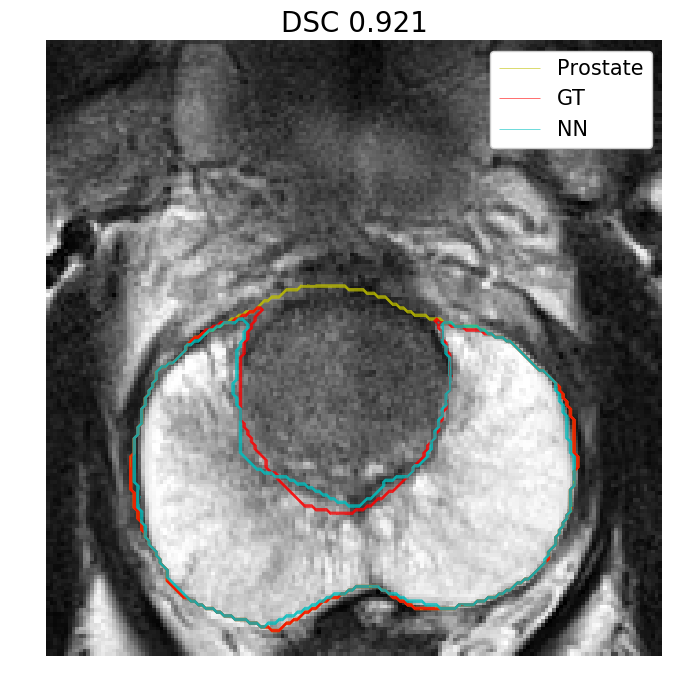
\includegraphics[totalheight=.2\textheight]{figures/results/PZ_Px_Challenge__P_yes_ROI_MAX_Case-0026.png}
%    \vspace{10mm}
%    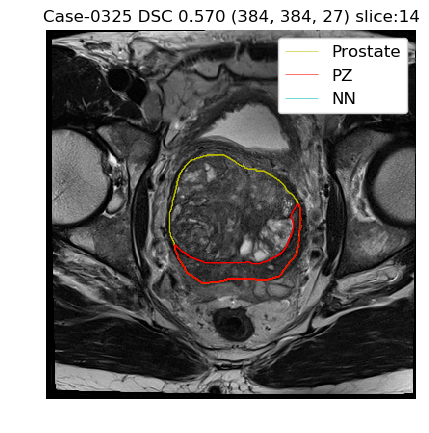
\includegraphics[totalheight=.2\textheight]{figures/results/PZ_Px_Challenge__P_yes_Original_MIN_Case-0325.png}
%    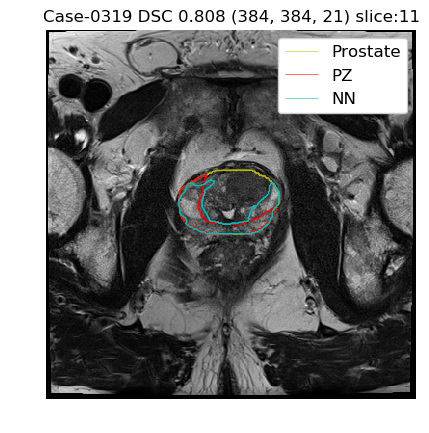
\includegraphics[totalheight=.2\textheight]{figures/results/PZ_Px_Challenge__P_yes_Original_MEAN_Case-0319.png}
%    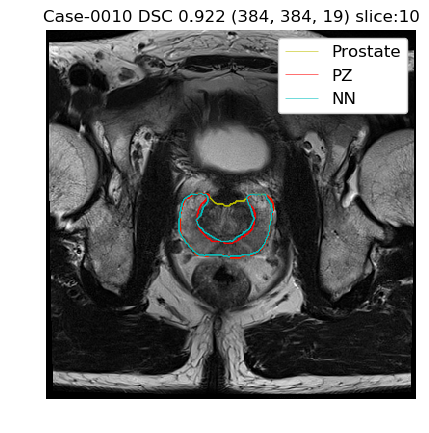
\includegraphics[totalheight=.2\textheight]{figures/results/PZ_Px_Challenge__P_yes_Original_MAX_Case-0010.png}
%    \vspace{10mm}
%    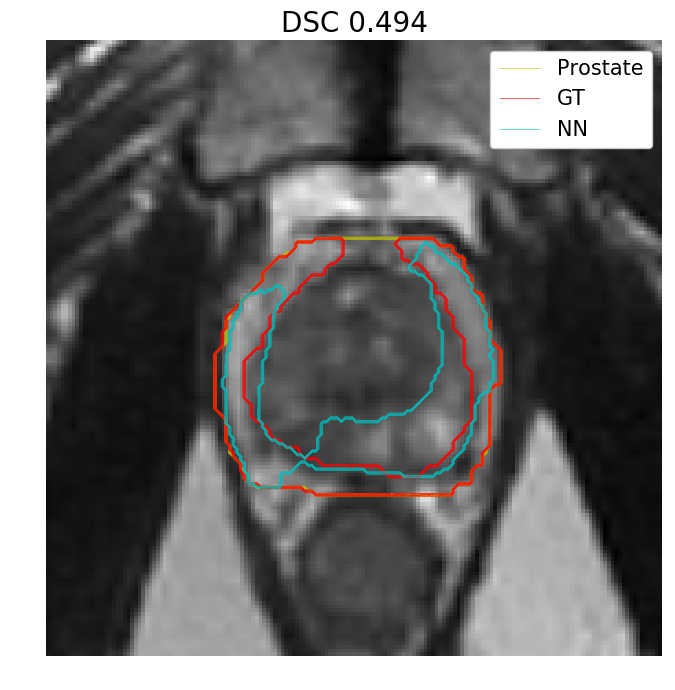
\includegraphics[totalheight=.2\textheight]{figures/results/PZ_GE__GE_yes_ROI_MIN_Case-0481.png}
%    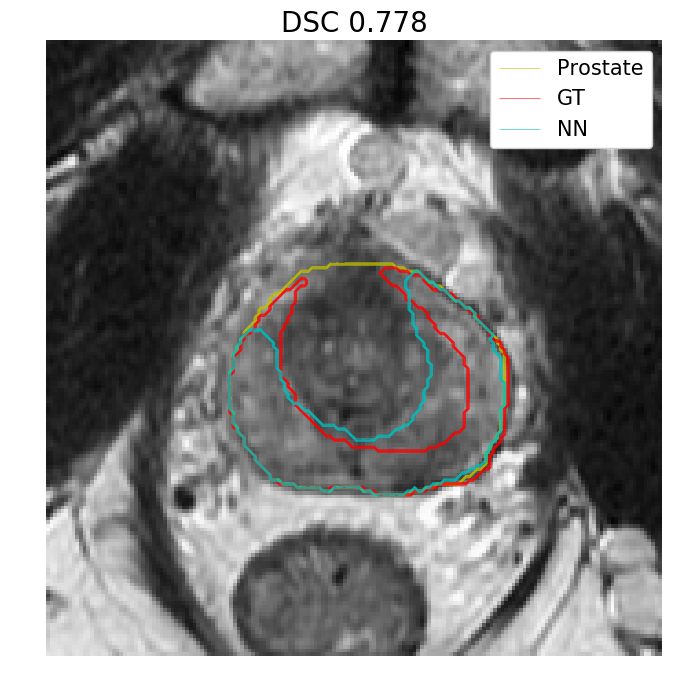
\includegraphics[totalheight=.2\textheight]{figures/results/PZ_GE__GE_yes_ROI_MEAN_Case-0462.png}
%    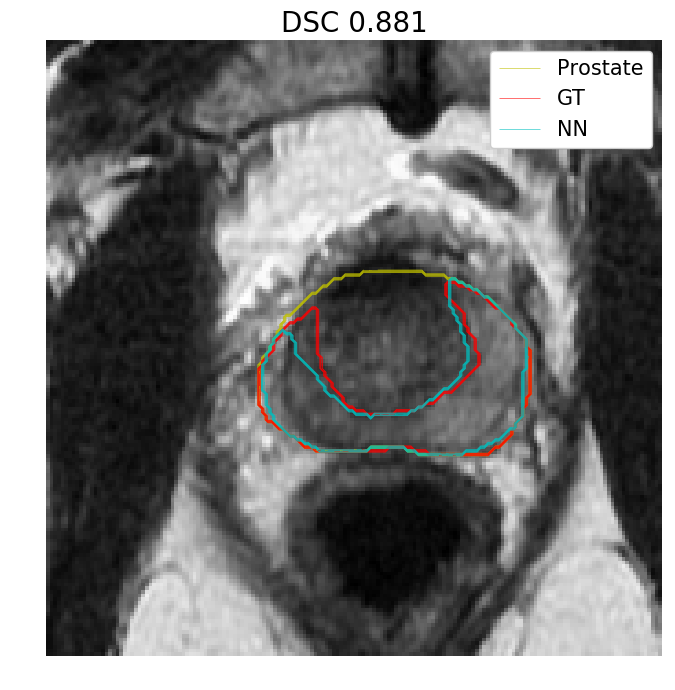
\includegraphics[totalheight=.2\textheight]{figures/results/PZ_GE__GE_yes_ROI_MAX_Case-0508.png}
%    \vspace{10mm}
%    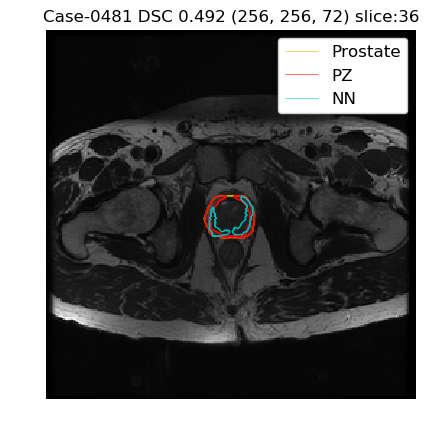
\includegraphics[totalheight=.2\textheight]{figures/results/PZ_GE__GE_yes_Original_MIN_Case-0481.png}
%    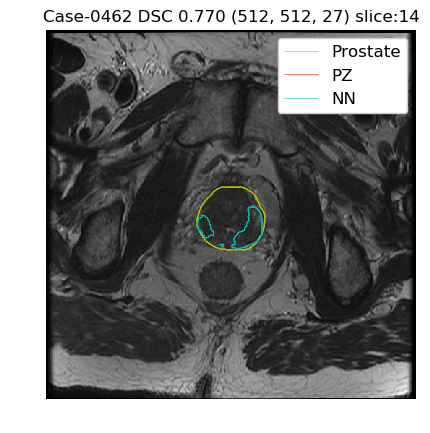
\includegraphics[totalheight=.2\textheight]{figures/results/PZ_GE__GE_yes_Original_MEAN_Case-0462.png}
%    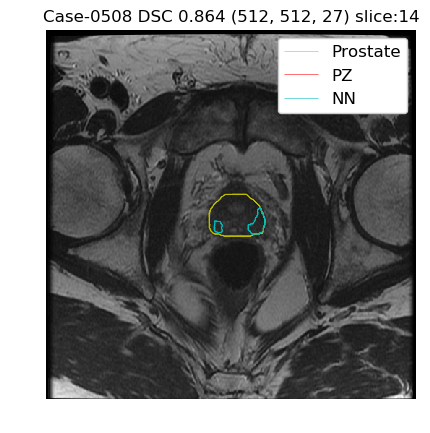
\includegraphics[totalheight=.2\textheight]{figures/results/PZ_GE__GE_yes_Original_MAX_Case-0508.png}
%    \label{fig:ressegpz}
%   \caption{PZ segmentations of Siemens (up) and GE (down) MRI vendors respectively. }
%\end{figure} 

%\begin{figure}[h]
    %\centering
    %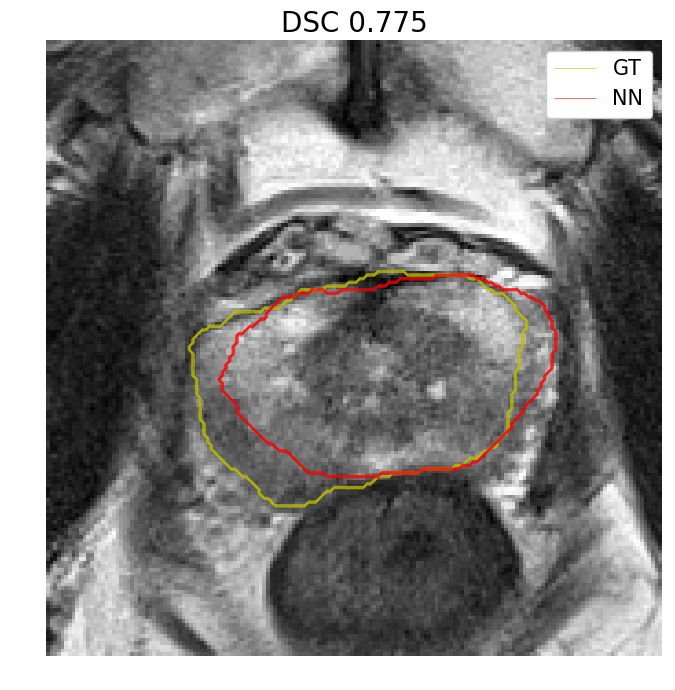
\includegraphics[totalheight=.2\textheight]{figures/results/Prostate_Px_Challenge__P_yes_ROI_MIN_Case-0128.png}
    %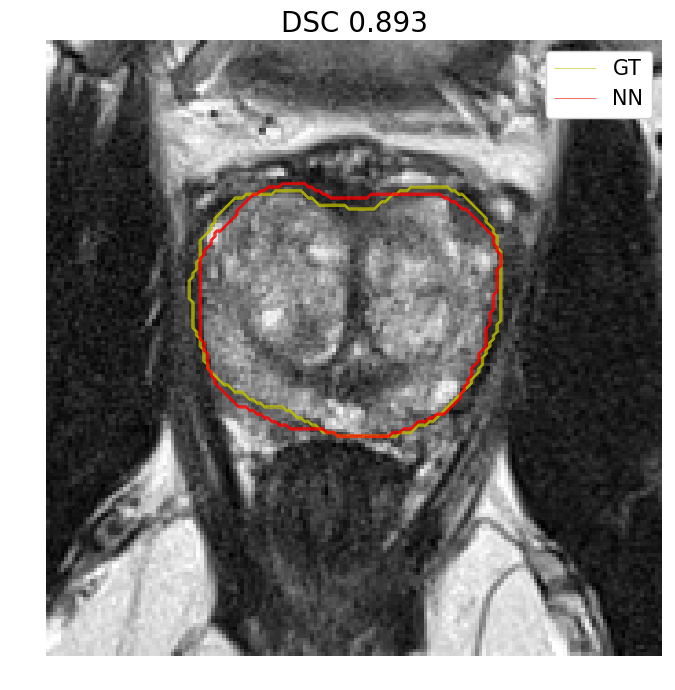
\includegraphics[totalheight=.2\textheight]{figures/results/Prostate_Px_Challenge__P_yes_ROI_MEAN_Case-0176.png}
    %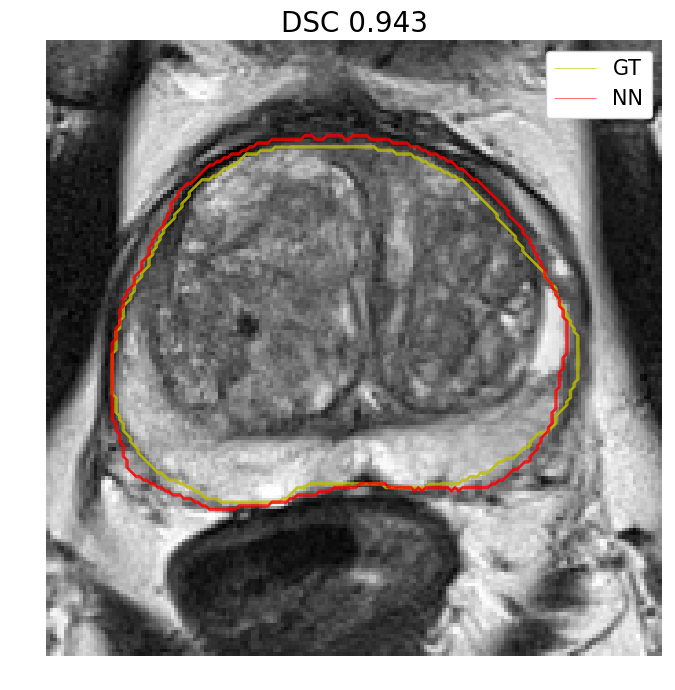
\includegraphics[totalheight=.2\textheight]{figures/results/Prostate_Px_Challenge__P_yes_ROI_MAX_Case-0337.png}
    %\vspace{10mm}
    %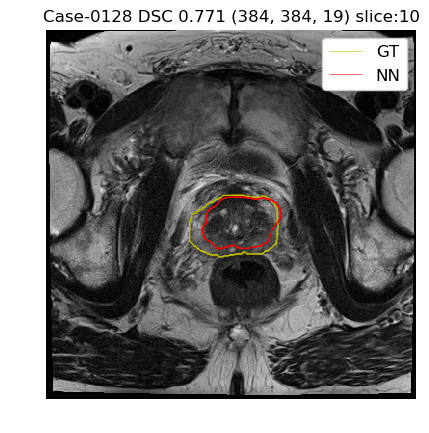
\includegraphics[totalheight=.2\textheight]{figures/results/Prostate_Px_Challenge__P_yes_Original_MIN_Case-0128.png}
    %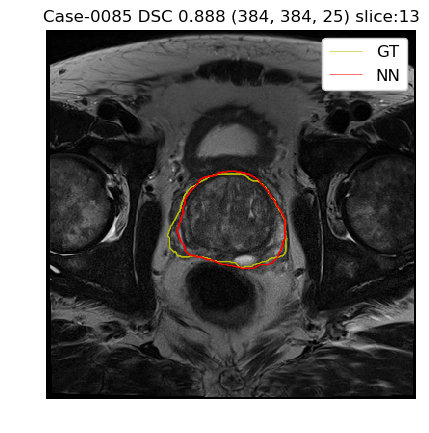
\includegraphics[totalheight=.2\textheight]{figures/results/Prostate_Px_Challenge__P_yes_Original_MEAN_Case-0085.png}
    %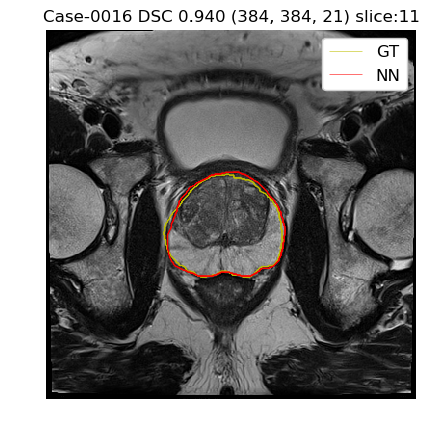
\includegraphics[totalheight=.2\textheight]{figures/results/Prostate_Px_Challenge__P_yes_Original_MAX_Case-0016.png}
    %\vspace{10mm}
    %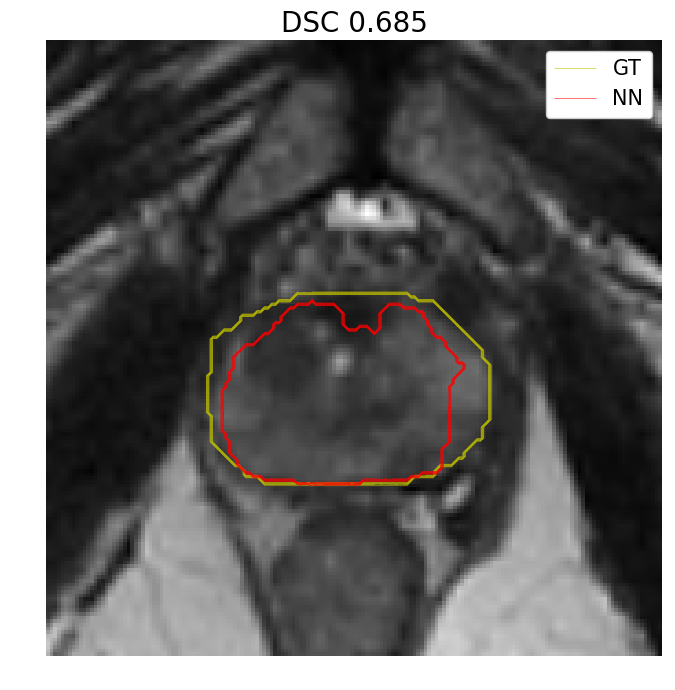
\includegraphics[totalheight=.2\textheight]{figures/results/Prostate_GE__GE_yes_ROI_MIN_Case-0518.png}
    %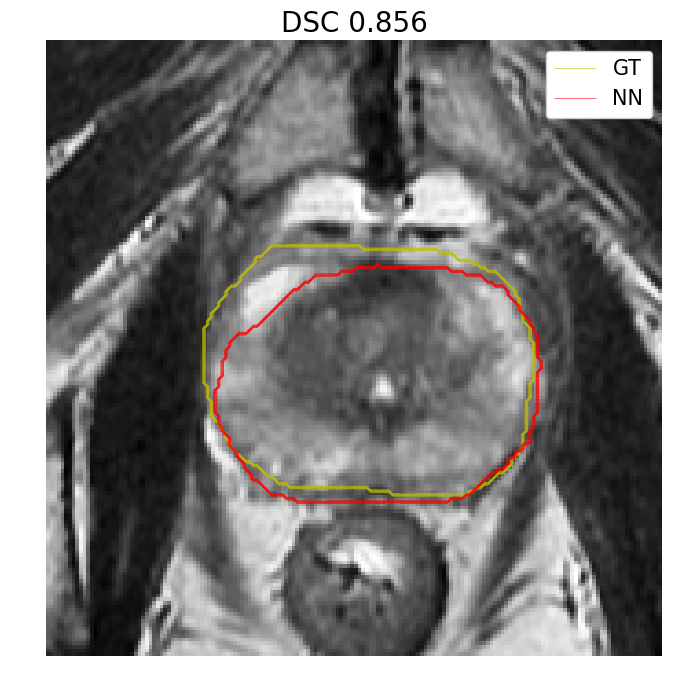
\includegraphics[totalheight=.2\textheight]{figures/results/Prostate_GE__GE_yes_ROI_MEAN_Case-0544.png}
    %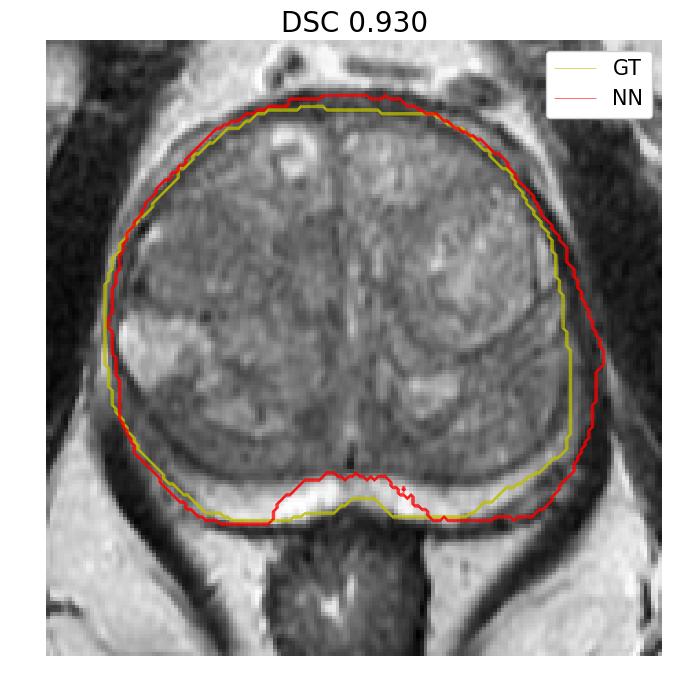
\includegraphics[totalheight=.2\textheight]{figures/results/Prostate_GE__GE_yes_ROI_MAX_Case-0537.png}
    %\vspace{10mm}
    %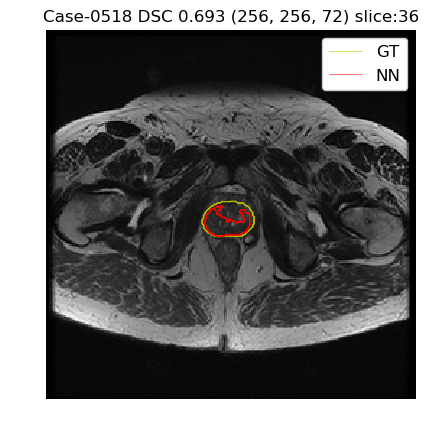
\includegraphics[totalheight=.2\textheight]{figures/results/Prostate_GE__GE_yes_Original_MIN_Case-0518.png}
    %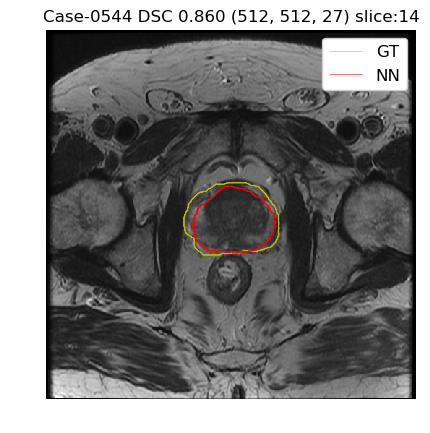
\includegraphics[totalheight=.2\textheight]{figures/results/Prostate_GE__GE_yes_Original_MEAN_Case-0544.png}
    %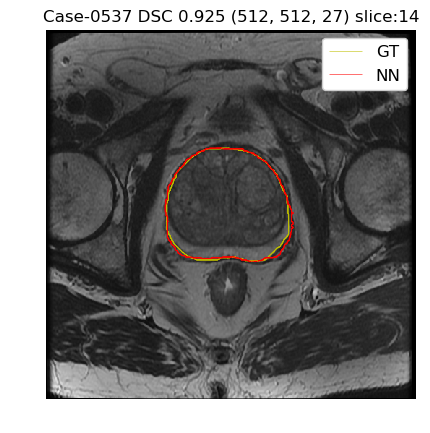
\includegraphics[totalheight=.2\textheight]{figures/results/Prostate_GE__GE_yes_Original_MAX_Case-0537.png}
    %\label{fig:resseg}
    %\caption{Prostate segmentations of Siemens (up) and GE (down) MRI vendors respectively. }
%\end{figure} 
